\documentclass[twoside]{book}

% Packages required by doxygen
\usepackage{fixltx2e}
\usepackage{calc}
\usepackage{doxygen}
\usepackage[export]{adjustbox} % also loads graphicx
\usepackage{graphicx}
\usepackage[utf8]{inputenc}
\usepackage{makeidx}
\usepackage{multicol}
\usepackage{multirow}
\PassOptionsToPackage{warn}{textcomp}
\usepackage{textcomp}
\usepackage[nointegrals]{wasysym}
\usepackage[table]{xcolor}

% Font selection
\usepackage[T1]{fontenc}
\usepackage[scaled=.90]{helvet}
\usepackage{courier}
\usepackage{amssymb}
\usepackage{sectsty}
\renewcommand{\familydefault}{\sfdefault}
\allsectionsfont{%
  \fontseries{bc}\selectfont%
  \color{darkgray}%
}
\renewcommand{\DoxyLabelFont}{%
  \fontseries{bc}\selectfont%
  \color{darkgray}%
}
\newcommand{\+}{\discretionary{\mbox{\scriptsize$\hookleftarrow$}}{}{}}

% Page & text layout
\usepackage{geometry}
\geometry{%
  a4paper,%
  top=2.5cm,%
  bottom=2.5cm,%
  left=2.5cm,%
  right=2.5cm%
}
\tolerance=750
\hfuzz=15pt
\hbadness=750
\setlength{\emergencystretch}{15pt}
\setlength{\parindent}{0cm}
\setlength{\parskip}{3ex plus 2ex minus 2ex}
\makeatletter
\renewcommand{\paragraph}{%
  \@startsection{paragraph}{4}{0ex}{-1.0ex}{1.0ex}{%
    \normalfont\normalsize\bfseries\SS@parafont%
  }%
}
\renewcommand{\subparagraph}{%
  \@startsection{subparagraph}{5}{0ex}{-1.0ex}{1.0ex}{%
    \normalfont\normalsize\bfseries\SS@subparafont%
  }%
}
\makeatother

% Headers & footers
\usepackage{fancyhdr}
\pagestyle{fancyplain}
\fancyhead[LE]{\fancyplain{}{\bfseries\thepage}}
\fancyhead[CE]{\fancyplain{}{}}
\fancyhead[RE]{\fancyplain{}{\bfseries\leftmark}}
\fancyhead[LO]{\fancyplain{}{\bfseries\rightmark}}
\fancyhead[CO]{\fancyplain{}{}}
\fancyhead[RO]{\fancyplain{}{\bfseries\thepage}}
\fancyfoot[LE]{\fancyplain{}{}}
\fancyfoot[CE]{\fancyplain{}{}}
\fancyfoot[RE]{\fancyplain{}{\bfseries\scriptsize Generated by Doxygen }}
\fancyfoot[LO]{\fancyplain{}{\bfseries\scriptsize Generated by Doxygen }}
\fancyfoot[CO]{\fancyplain{}{}}
\fancyfoot[RO]{\fancyplain{}{}}
\renewcommand{\footrulewidth}{0.4pt}
\renewcommand{\chaptermark}[1]{%
  \markboth{#1}{}%
}
\renewcommand{\sectionmark}[1]{%
  \markright{\thesection\ #1}%
}

% Indices & bibliography
\usepackage{natbib}
\usepackage[titles]{tocloft}
\setcounter{tocdepth}{3}
\setcounter{secnumdepth}{5}
\makeindex

% Hyperlinks (required, but should be loaded last)
\usepackage{ifpdf}
\ifpdf
  \usepackage[pdftex,pagebackref=true]{hyperref}
\else
  \usepackage[ps2pdf,pagebackref=true]{hyperref}
\fi
\hypersetup{%
  colorlinks=true,%
  linkcolor=blue,%
  citecolor=blue,%
  unicode%
}

% Custom commands
\newcommand{\clearemptydoublepage}{%
  \newpage{\pagestyle{empty}\cleardoublepage}%
}

\usepackage{caption}
\captionsetup{labelsep=space,justification=centering,font={bf},singlelinecheck=off,skip=4pt,position=top}

%===== C O N T E N T S =====

\begin{document}

% Titlepage & ToC
\hypersetup{pageanchor=false,
             bookmarksnumbered=true,
             pdfencoding=unicode
            }
\pagenumbering{roman}
\begin{titlepage}
\vspace*{7cm}
\begin{center}%
{\Large D\+S\+M\+DE \\[1ex]\large 0.\+1 }\\
\vspace*{1cm}
{\large Generated by Doxygen 1.8.11}\\
\end{center}
\end{titlepage}
\clearemptydoublepage
\tableofcontents
\clearemptydoublepage
\pagenumbering{arabic}
\hypersetup{pageanchor=true}

%--- Begin generated contents ---
\chapter{Namespace Index}
\section{Packages}
Here are the packages with brief descriptions (if available)\+:\begin{DoxyCompactList}
\item\contentsline{section}{\hyperlink{namespacedriver}{driver} }{\pageref{namespacedriver}}{}
\item\contentsline{section}{\hyperlink{namespacescanner}{scanner} }{\pageref{namespacescanner}}{}
\end{DoxyCompactList}

\chapter{Hierarchical Index}
\section{Class Hierarchy}
This inheritance list is sorted roughly, but not completely, alphabetically\+:\begin{DoxyCompactList}
\item \contentsline{section}{driver.\+Administration}{\pageref{classdriver_1_1Administration}}{}
\item \contentsline{section}{driver.\+driver}{\pageref{classdriver_1_1driver}}{}
\item \contentsline{section}{parser.\+First\+Follow}{\pageref{classparser_1_1FirstFollow}}{}
\item \contentsline{section}{parser.\+Parser}{\pageref{classparser_1_1Parser}}{}
\item \contentsline{section}{scanner.\+Scan\+Me}{\pageref{classscanner_1_1ScanMe}}{}
\item \contentsline{section}{scanner.\+Symbol}{\pageref{enumscanner_1_1Symbol}}{}
\item \contentsline{section}{symbol\+Table.\+Symbol\+Table}{\pageref{classsymbolTable_1_1SymbolTable}}{}
\item \contentsline{section}{scanner.\+Token}{\pageref{classscanner_1_1Token}}{}
\item J\+Frame\begin{DoxyCompactList}
\item \contentsline{section}{driver.\+Driver\+Window}{\pageref{classdriver_1_1DriverWindow}}{}
\end{DoxyCompactList}
\end{DoxyCompactList}

\chapter{Class Index}
\section{Class List}
Here are the classes, structs, unions and interfaces with brief descriptions\+:\begin{DoxyCompactList}
\item\contentsline{section}{\hyperlink{classdriver_1_1driver}{driver.\+driver} }{\pageref{classdriver_1_1driver}}{}
\item\contentsline{section}{\hyperlink{classdriver_1_1DriverWindow}{driver.\+Driver\+Window} }{\pageref{classdriver_1_1DriverWindow}}{}
\item\contentsline{section}{\hyperlink{classscanner_1_1Scanner}{scanner.\+Scanner} }{\pageref{classscanner_1_1Scanner}}{}
\end{DoxyCompactList}

\chapter{File Index}
\section{File List}
Here is a list of all files with brief descriptions\+:\begin{DoxyCompactList}
\item\contentsline{section}{src/driver/\hyperlink{driver_8java}{driver.\+java} \\*Drives the project }{\pageref{driver_8java}}{}
\item\contentsline{section}{src/driver/\hyperlink{DriverWindow_8java}{Driver\+Window.\+java} \\*This the driver class Provides UI for user to choose file from dialog }{\pageref{DriverWindow_8java}}{}
\item\contentsline{section}{src/scanner/\hyperlink{Scanner_8java}{Scanner.\+java} \\*This the scanner class This class generates meaningful tokens from source file }{\pageref{Scanner_8java}}{}
\end{DoxyCompactList}

\chapter{Namespace Documentation}
\hypertarget{namespacedriver}{}\section{Package driver}
\label{namespacedriver}\index{driver@{driver}}
\subsection*{Classes}
\begin{DoxyCompactItemize}
\item 
class \hyperlink{classdriver_1_1Administration}{Administration}
\item 
class \hyperlink{classdriver_1_1driver}{driver}
\item 
class \hyperlink{classdriver_1_1DriverWindow}{Driver\+Window}
\end{DoxyCompactItemize}

\hypertarget{namespacescanner}{}\section{Package scanner}
\label{namespacescanner}\index{scanner@{scanner}}
\subsection*{Classes}
\begin{DoxyCompactItemize}
\item 
class \hyperlink{classscanner_1_1ScanMe}{Scan\+Me}
\item 
enum \hyperlink{enumscanner_1_1Symbol}{Symbol}
\item 
class \hyperlink{classscanner_1_1Token}{Token}
\end{DoxyCompactItemize}

\chapter{Class Documentation}
\hypertarget{classdriver_1_1driver}{}\section{driver.\+driver Class Reference}
\label{classdriver_1_1driver}\index{driver.\+driver@{driver.\+driver}}
\subsection*{Static Public Member Functions}
\begin{DoxyCompactItemize}
\item 
static void \hyperlink{classdriver_1_1driver_ab4bbf6027065ef2d09f1e20f8346d2bf}{main} (String\mbox{[}$\,$\mbox{]} args)
\end{DoxyCompactItemize}
\subsection*{Public Attributes}
\begin{DoxyCompactItemize}
\item 
int \hyperlink{classdriver_1_1driver_a171341186cc3c3a33ce7f44a938d9bcd}{var}
\end{DoxyCompactItemize}


\subsection{Detailed Description}
This is the main file. Program starts from main file 

\subsection{Member Function Documentation}
\index{driver\+::driver@{driver\+::driver}!main@{main}}
\index{main@{main}!driver\+::driver@{driver\+::driver}}
\subsubsection[{\texorpdfstring{main(\+String[] args)}{main(String[] args)}}]{\setlength{\rightskip}{0pt plus 5cm}static void driver.\+driver.\+main (
\begin{DoxyParamCaption}
\item[{String\mbox{[}$\,$\mbox{]}}]{args}
\end{DoxyParamCaption}
)\hspace{0.3cm}{\ttfamily [static]}}\hypertarget{classdriver_1_1driver_ab4bbf6027065ef2d09f1e20f8346d2bf}{}\label{classdriver_1_1driver_ab4bbf6027065ef2d09f1e20f8346d2bf}

\begin{DoxyParams}{Parameters}
{\em args} & \\
\hline
\end{DoxyParams}


\subsection{Member Data Documentation}
\index{driver\+::driver@{driver\+::driver}!var@{var}}
\index{var@{var}!driver\+::driver@{driver\+::driver}}
\subsubsection[{\texorpdfstring{var}{var}}]{\setlength{\rightskip}{0pt plus 5cm}int driver.\+driver.\+var}\hypertarget{classdriver_1_1driver_a171341186cc3c3a33ce7f44a938d9bcd}{}\label{classdriver_1_1driver_a171341186cc3c3a33ce7f44a938d9bcd}
this is a variable 

The documentation for this class was generated from the following file\+:\begin{DoxyCompactItemize}
\item 
src/driver/\hyperlink{driver_8java}{driver.\+java}\end{DoxyCompactItemize}

\hypertarget{classdriver_1_1DriverWindow}{}\section{driver.\+Driver\+Window Class Reference}
\label{classdriver_1_1DriverWindow}\index{driver.\+Driver\+Window@{driver.\+Driver\+Window}}
Inheritance diagram for driver.\+Driver\+Window\+:\begin{figure}[H]
\begin{center}
\leavevmode
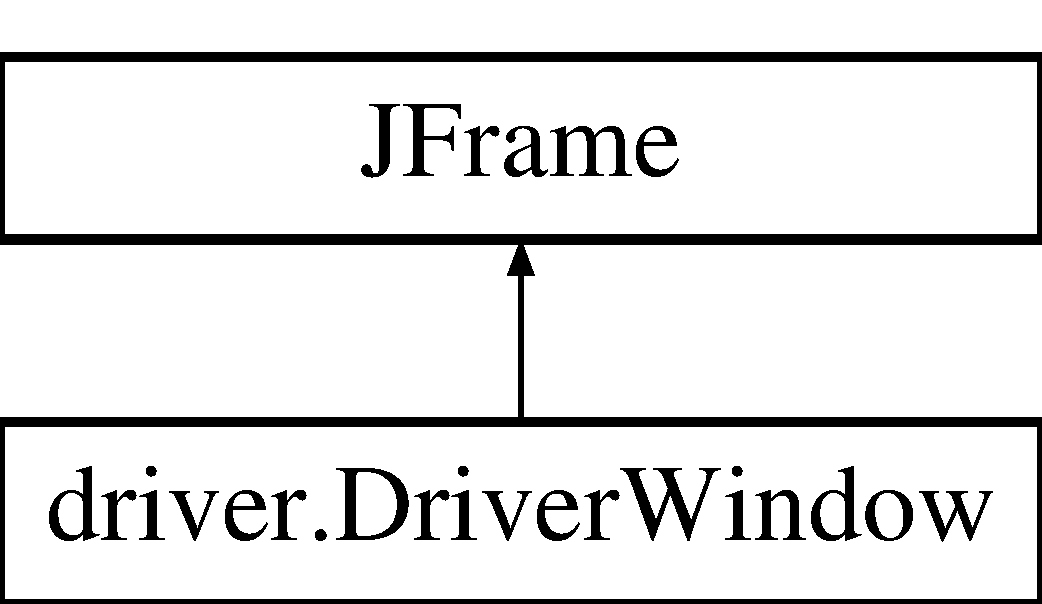
\includegraphics[height=2.000000cm]{classdriver_1_1DriverWindow}
\end{center}
\end{figure}
\subsection*{Public Member Functions}
\begin{DoxyCompactItemize}
\item 
\hyperlink{classdriver_1_1DriverWindow_acc35b31088a5ffe1543c28462b56194f}{Driver\+Window} ()
\end{DoxyCompactItemize}
\subsection*{Static Public Member Functions}
\begin{DoxyCompactItemize}
\item 
static void \hyperlink{classdriver_1_1DriverWindow_af743a70776a96562bbfb500b93a2e742}{main} (String\mbox{[}$\,$\mbox{]} args)
\end{DoxyCompactItemize}
\subsection*{Public Attributes}
\begin{DoxyCompactItemize}
\item 
File\+Reader \hyperlink{classdriver_1_1DriverWindow_a463a3d013ea4e8f95c818b2f7a7842d0}{source\+File} = null
\begin{DoxyCompactList}\small\item\em source\+File object is the reader of source file \end{DoxyCompactList}\end{DoxyCompactItemize}
\subsection*{Private Member Functions}
\begin{DoxyCompactItemize}
\item 
void \hyperlink{classdriver_1_1DriverWindow_a0513dffb45726e4a9ef3db30c3aec57e}{open\+File\+Stream} (String absolute\+Path)
\end{DoxyCompactItemize}
\subsection*{Private Attributes}
\begin{DoxyCompactItemize}
\item 
J\+Panel \hyperlink{classdriver_1_1DriverWindow_ac02788f4ca5e699895e910d672237baa}{content\+Pane}
\item 
J\+Text\+Field \hyperlink{classdriver_1_1DriverWindow_a28cd643f483a25f1793d57daae2813b1}{text\+Field}
\end{DoxyCompactItemize}


\subsection{Constructor \& Destructor Documentation}
\index{driver\+::\+Driver\+Window@{driver\+::\+Driver\+Window}!Driver\+Window@{Driver\+Window}}
\index{Driver\+Window@{Driver\+Window}!driver\+::\+Driver\+Window@{driver\+::\+Driver\+Window}}
\subsubsection[{\texorpdfstring{Driver\+Window()}{DriverWindow()}}]{\setlength{\rightskip}{0pt plus 5cm}driver.\+Driver\+Window.\+Driver\+Window (
\begin{DoxyParamCaption}
{}
\end{DoxyParamCaption}
)}\hypertarget{classdriver_1_1DriverWindow_acc35b31088a5ffe1543c28462b56194f}{}\label{classdriver_1_1DriverWindow_acc35b31088a5ffe1543c28462b56194f}
Create the frame. 

\subsection{Member Function Documentation}
\index{driver\+::\+Driver\+Window@{driver\+::\+Driver\+Window}!main@{main}}
\index{main@{main}!driver\+::\+Driver\+Window@{driver\+::\+Driver\+Window}}
\subsubsection[{\texorpdfstring{main(\+String[] args)}{main(String[] args)}}]{\setlength{\rightskip}{0pt plus 5cm}static void driver.\+Driver\+Window.\+main (
\begin{DoxyParamCaption}
\item[{String\mbox{[}$\,$\mbox{]}}]{args}
\end{DoxyParamCaption}
)\hspace{0.3cm}{\ttfamily [static]}}\hypertarget{classdriver_1_1DriverWindow_af743a70776a96562bbfb500b93a2e742}{}\label{classdriver_1_1DriverWindow_af743a70776a96562bbfb500b93a2e742}
Launch the application. \index{driver\+::\+Driver\+Window@{driver\+::\+Driver\+Window}!open\+File\+Stream@{open\+File\+Stream}}
\index{open\+File\+Stream@{open\+File\+Stream}!driver\+::\+Driver\+Window@{driver\+::\+Driver\+Window}}
\subsubsection[{\texorpdfstring{open\+File\+Stream(\+String absolute\+Path)}{openFileStream(String absolutePath)}}]{\setlength{\rightskip}{0pt plus 5cm}void driver.\+Driver\+Window.\+open\+File\+Stream (
\begin{DoxyParamCaption}
\item[{String}]{absolute\+Path}
\end{DoxyParamCaption}
)\hspace{0.3cm}{\ttfamily [private]}}\hypertarget{classdriver_1_1DriverWindow_a0513dffb45726e4a9ef3db30c3aec57e}{}\label{classdriver_1_1DriverWindow_a0513dffb45726e4a9ef3db30c3aec57e}

\begin{DoxyParams}{Parameters}
{\em absolute\+Path} & opens file using file reader and the absolute path of the chosen file \\
\hline
\end{DoxyParams}


\subsection{Member Data Documentation}
\index{driver\+::\+Driver\+Window@{driver\+::\+Driver\+Window}!content\+Pane@{content\+Pane}}
\index{content\+Pane@{content\+Pane}!driver\+::\+Driver\+Window@{driver\+::\+Driver\+Window}}
\subsubsection[{\texorpdfstring{content\+Pane}{contentPane}}]{\setlength{\rightskip}{0pt plus 5cm}J\+Panel driver.\+Driver\+Window.\+content\+Pane\hspace{0.3cm}{\ttfamily [private]}}\hypertarget{classdriver_1_1DriverWindow_ac02788f4ca5e699895e910d672237baa}{}\label{classdriver_1_1DriverWindow_ac02788f4ca5e699895e910d672237baa}
\index{driver\+::\+Driver\+Window@{driver\+::\+Driver\+Window}!source\+File@{source\+File}}
\index{source\+File@{source\+File}!driver\+::\+Driver\+Window@{driver\+::\+Driver\+Window}}
\subsubsection[{\texorpdfstring{source\+File}{sourceFile}}]{\setlength{\rightskip}{0pt plus 5cm}File\+Reader driver.\+Driver\+Window.\+source\+File = null}\hypertarget{classdriver_1_1DriverWindow_a463a3d013ea4e8f95c818b2f7a7842d0}{}\label{classdriver_1_1DriverWindow_a463a3d013ea4e8f95c818b2f7a7842d0}


source\+File object is the reader of source file 

\index{driver\+::\+Driver\+Window@{driver\+::\+Driver\+Window}!text\+Field@{text\+Field}}
\index{text\+Field@{text\+Field}!driver\+::\+Driver\+Window@{driver\+::\+Driver\+Window}}
\subsubsection[{\texorpdfstring{text\+Field}{textField}}]{\setlength{\rightskip}{0pt plus 5cm}J\+Text\+Field driver.\+Driver\+Window.\+text\+Field\hspace{0.3cm}{\ttfamily [private]}}\hypertarget{classdriver_1_1DriverWindow_a28cd643f483a25f1793d57daae2813b1}{}\label{classdriver_1_1DriverWindow_a28cd643f483a25f1793d57daae2813b1}


The documentation for this class was generated from the following file\+:\begin{DoxyCompactItemize}
\item 
src/driver/\hyperlink{DriverWindow_8java}{Driver\+Window.\+java}\end{DoxyCompactItemize}

\hypertarget{classscanner_1_1Scanner}{}\section{scanner.\+Scanner Class Reference}
\label{classscanner_1_1Scanner}\index{scanner.\+Scanner@{scanner.\+Scanner}}
\subsection*{Public Member Functions}
\begin{DoxyCompactItemize}
\item 
\hyperlink{classscanner_1_1Scanner_a344b0265cf89d07cfa090f681453a39b}{Scanner} (File\+Reader src\+File)
\end{DoxyCompactItemize}


\subsection{Constructor \& Destructor Documentation}
\index{scanner\+::\+Scanner@{scanner\+::\+Scanner}!Scanner@{Scanner}}
\index{Scanner@{Scanner}!scanner\+::\+Scanner@{scanner\+::\+Scanner}}
\subsubsection[{\texorpdfstring{Scanner(\+File\+Reader src\+File)}{Scanner(FileReader srcFile)}}]{\setlength{\rightskip}{0pt plus 5cm}scanner.\+Scanner.\+Scanner (
\begin{DoxyParamCaption}
\item[{File\+Reader}]{src\+File}
\end{DoxyParamCaption}
)}\hypertarget{classscanner_1_1Scanner_a344b0265cf89d07cfa090f681453a39b}{}\label{classscanner_1_1Scanner_a344b0265cf89d07cfa090f681453a39b}


The documentation for this class was generated from the following file\+:\begin{DoxyCompactItemize}
\item 
src/scanner/\hyperlink{Scanner_8java}{Scanner.\+java}\end{DoxyCompactItemize}

\chapter{File Documentation}
\hypertarget{driver_8java}{}\section{src/driver/driver.java File Reference}
\label{driver_8java}\index{src/driver/driver.\+java@{src/driver/driver.\+java}}


Drives the project.  


\subsection*{Classes}
\begin{DoxyCompactItemize}
\item 
class \hyperlink{classdriver_1_1driver}{driver.\+driver}
\end{DoxyCompactItemize}
\subsection*{Packages}
\begin{DoxyCompactItemize}
\item 
package \hyperlink{namespacedriver}{driver}
\end{DoxyCompactItemize}


\subsection{Detailed Description}
Drives the project. 

This file is the driver file. From this point the project initiates. \begin{DoxyAuthor}{Author}
Ahamad Imtiaz Khan 
\end{DoxyAuthor}
\begin{DoxyVersion}{Version}
1.\+0 
\end{DoxyVersion}
\begin{DoxyDate}{Date}
2016 
\end{DoxyDate}

\hypertarget{DriverWindow_8java}{}\section{src/driver/\+Driver\+Window.java File Reference}
\label{DriverWindow_8java}\index{src/driver/\+Driver\+Window.\+java@{src/driver/\+Driver\+Window.\+java}}


This the driver class Provides UI for user to choose file from dialog.  


\subsection*{Classes}
\begin{DoxyCompactItemize}
\item 
class \hyperlink{classdriver_1_1DriverWindow}{driver.\+Driver\+Window}
\end{DoxyCompactItemize}
\subsection*{Packages}
\begin{DoxyCompactItemize}
\item 
package \hyperlink{namespacedriver}{driver}
\end{DoxyCompactItemize}


\subsection{Detailed Description}
This the driver class Provides UI for user to choose file from dialog. 

\begin{DoxyAuthor}{Author}
Ahamad Imtiaz Khan 
\end{DoxyAuthor}
\begin{DoxyVersion}{Version}
0.\+1 
\end{DoxyVersion}

\hypertarget{Scanner_8java}{}\section{src/scanner/\+Scanner.java File Reference}
\label{Scanner_8java}\index{src/scanner/\+Scanner.\+java@{src/scanner/\+Scanner.\+java}}


This the scanner class This class generates meaningful tokens from source file.  


\subsection*{Classes}
\begin{DoxyCompactItemize}
\item 
class \hyperlink{classscanner_1_1Scanner}{scanner.\+Scanner}
\end{DoxyCompactItemize}
\subsection*{Packages}
\begin{DoxyCompactItemize}
\item 
package \hyperlink{namespacescanner}{scanner}
\end{DoxyCompactItemize}


\subsection{Detailed Description}
This the scanner class This class generates meaningful tokens from source file. 

\begin{DoxyAuthor}{Author}
Ahamad Imtiaz Khan 
\end{DoxyAuthor}

%--- End generated contents ---

% Index
\backmatter
\newpage
\phantomsection
\clearemptydoublepage
\addcontentsline{toc}{chapter}{Index}
\printindex

\end{document}
